\chapter*{Úvod}
\renewcommand{\chaptername}{Úvod}

% Bronchoalveolární laváž (BAL) je invazivní diagnostický postup, který se používá k diagnostice a monitorování plicních onemocnění.
Bronchoalveolární laváž (BAL) je invazivní vyšetření plic, které se provádí za účelem diagnostiky a monitorování plicních onemocnění.
Během tohoto zákroku je do plicních sklípků zavedena tekutina, která se následně odsaje a analyzuje (BAL fluid nebo také BALF, česky BAT).
Z této tekutiny je cílem získat diferenciální počet buněk jednotlivých typů buněk (příklad výstupu lze vidět na obrázku \ref{fig:tabulka_dif_pocty}).
Automatizovaná analýza pomocí počítačového zpracování obrazu může zrychlit diagnostiku a zlepšit přesnost.

\begin{figure}[H]
    \centering
    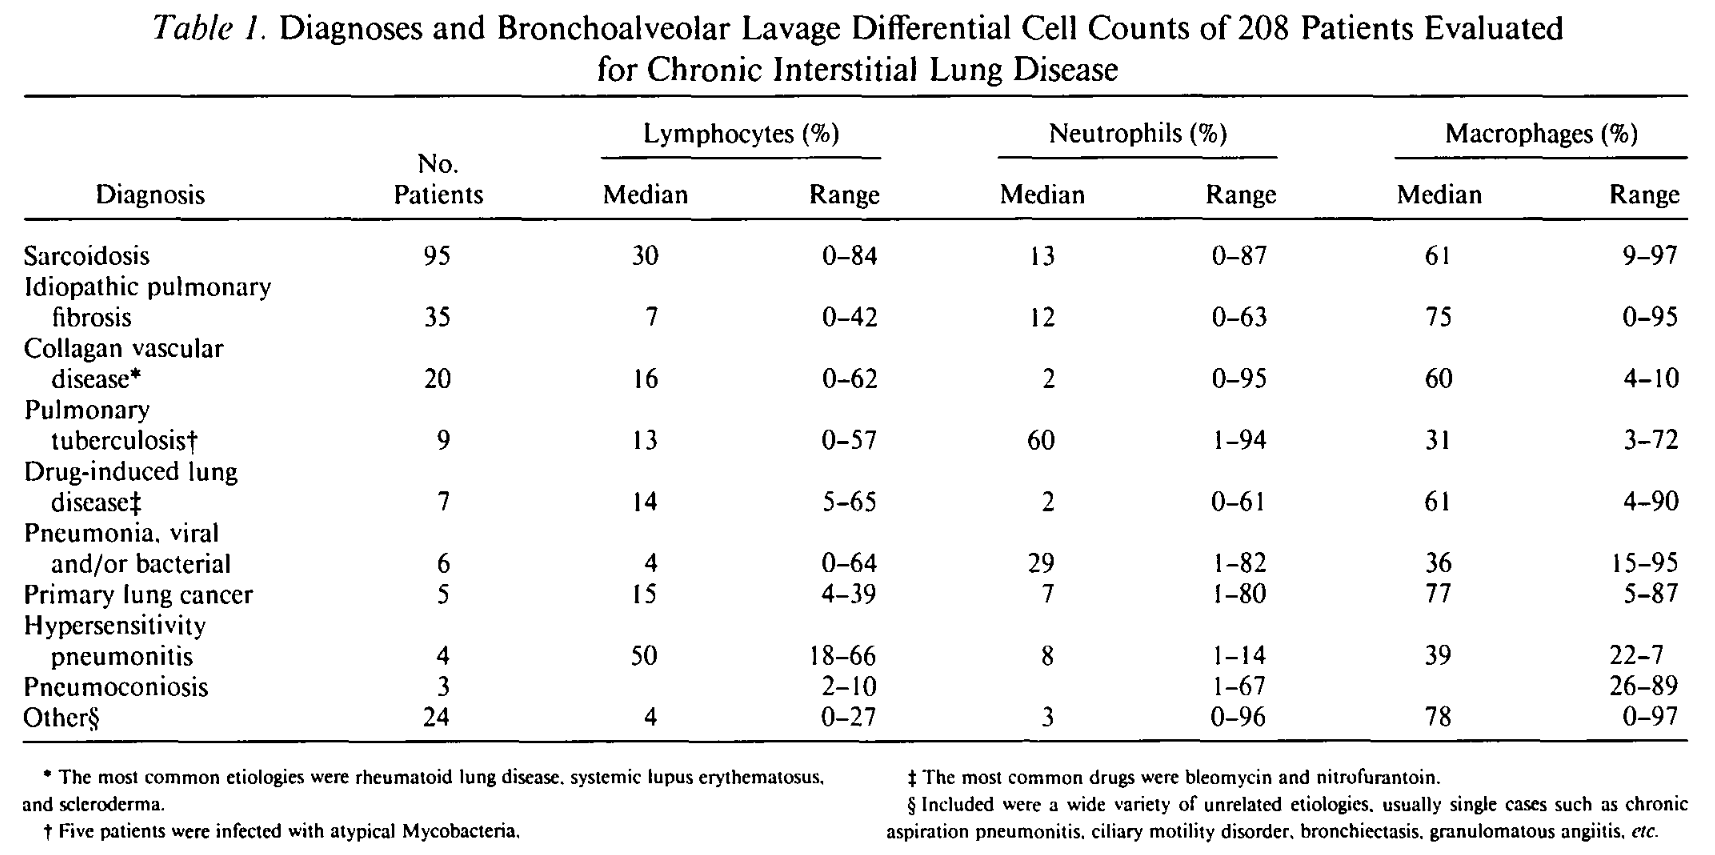
\includegraphics[width=\textwidth]{static/obrazky/tabulka_dif_pocty.png}
    \caption{Diagnostika podle diferenciálního počtu buněk. Převzato z \cite{Check19851201}.}
    \label{fig:tabulka_dif_pocty}
\end{figure}

V oblasti segmentace buněk a automatizované analýzy cytologických snímků bylo provedeno několik studií zaměřených na různé metody a přístupy. Například v práci \cite{Caicedo2019} autoři analyzovali využití hlubokého učení pro segmentaci a klasifikaci buněk v mikroskopických snímcích, přičemž využili konvoluční neuronové sítě (CNN) a metody transferového učení k dosažení vysoké přesnosti. Další výzkum \cite{Ronneberger2015} se zaměřil na použití U-Net architektury pro segmentaci buněk v biomedicínských obrazech, což vedlo ke značnému pokroku v oblasti automatizovaného zpracování obrazu. Specificky v oblasti bronchoalveolární laváže existují studie, které se snaží o automatizaci diferenciálního počtu buněk pomocí strojového učení a zpracování obrazu \cite{Smith2021}, kde byly testovány různé přístupy k detekci a klasifikaci buněk v BALF vzorcích. Tyto práce ukazují, že kombinace pokročilých metod zpracování obrazu a hlubokého učení může významně přispět k automatizaci diagnostiky v cytologii a patologii.



Základem zpracování obrazu je segmentace, jejímž cílem je detekovat a rozlišit od sebe jednotlivé buňky a jádra, případně odstranit objekty, které nejsou předmětem zkoumání.
Tento úkol je v oblasti analýzy snímků buněk často obtížný.
Během zpracování je třeba se vypořádat s řadou problémů, jako jsou například překrývající se buňky, šum a v neposlední řadě i samotná kvalita snímků.
Buňky samotné mohou mít různé tvary a velikost. 
% Metody byly vybrány na základě předešlých prací \cite{FRIDRICH2022thesis}\cite{FRIDRICH2024thesis}.
% Součástí je jejich implementace a porovnání.
V této práci jsou v rámci oblastí segmentace jader a cytoplasmy buněk použity a porovnány algoritmy Watershed a SVM.

Hlavním cílem této práce je v segmentovaném snímku kolem buněk vytvořit bounding boxy tak, aby z jednotlivých buněk mohla být vygenerována datová sada.
Tato sada bude následně použita například pro trénování konvolučních neuronových sítí, které se využívají pro klasifikaci buněk.

Práce je členěna na teoretickou část, ve které jsou popsány použíté metody pro předzpracování, následnou segmentaci obrazu a vybrané metriky pro vyhodnocení kvality segmentace.
V následující praktické části je nejdříve věnována kapitola porovnání dvou použítých metod pro segmentaci buněk.
Následně je popsána implementace a výsledky detekce buněk a jader pomocí algoritmu watershed.
V záverečné kapitole je popsán proces vytváření bounding boxů kolem buněk.
% Pro klasifikaci se nejčastěji používají metody strojového učení, jako například konvoluční neuronové sítě.

% https://onlinelibrary.wiley.com/doi/epdf/10.1002/cyto.a.23984

% citovat Robust Nucleus/Cell Detection and Segmentation in Digital Pathology and Microscopy Images: A Comprehensive Review??